% % % % % % % % % % % % % % % % % % % % % % % % % % % % % % % % % % % % %
% Chapter: Experiment 1
% % % % % % % % % % % % % % % % % % % % % % % % % % % % % % % % % % % % %
\chapter{Experiment 1: Using random input}
\label{cpt:experiment1}
\pinfo{Props to test cases, implication returns True}
The properties that we defined in \autoref{cpt:properties} are translated into
test cases as described in \autoref{cpt:testmechanics}. In this experiment, we
expect to find some bugs that were unknown before by using the test framework.
When we have triggered some bugs, an investigation is needed to check what the
cause is of that bug. Next, we can categorize the bugs found to come to an
answer to this research question:\rqThree{}

% % % % % % % % % % % % % % % % % % % % % % % % % % % % % % % % % % % % %
% Section: Method
\section{Method}
%\label{sec:initial_case}
\pinfo{Like QuickCheck, recall cycle shortly}
In the first experiment, each property will be tested 100 times with random
input values. This means that if the property holds for 100 tests, it is
reported to be successfully satisfying the property. This is a similar approach
compared to what \textit{QuickCheck} does when checking properties. Unlike
\textit{QuickCheck}, the test framework does not shrink the input values to come
with minimum values for which the case fails. Instead, it will just report the
values that were used when the property failed.

% % % % % % % % % % % % % % % % % % % % % % % % % % % % % % % % % % % % %
% Section: Results
\section{Results}
Two runs are being done to detect bugs in the generator in this experiment
because the first run terminated quickly. The test framework was unable to
proceed in testing every property in this run.

% % % % % % % % % % % % %
% Subsection: First run
\subsection{First run}
\pinfo{Termination, compile error due to library}
The first run results into a termination of the run due to a compile error in the generated system. Although we made the assumption that the generated system should be compilable, this error came from a property definition that was expected to hold, namely \textit{AssociativeMultiplicationInteger1}. Which is why we can consider this as an error that is found when using the test framework. The error describes that an overloaded method cannot be applied to the \textit{Money} type, as shown in \autoref{lst:ch5_firstrun_termination_log}.
% Listing
\begin{sourcecode}[!ht]
\begin{lstlisting}[language=Log]
[error] MoneySpec.scala:316: overloaded method value * with alternatives:
[error]   (x: Double)Double <and>
[error]   (x: Float)Float <and>
[error]   (x: Long)Long <and>
[error]   (x: Int)Int <and>
[error]   (x: Char)Int <and>
[error]   (x: Short)Int <and>
[error]   (x: Byte)Int
[error]  cannot be applied to (squants.market.Money)
[error]           Initialised(Data(result = Some(((((x * y)) * z) == (x * ((y * z)))))))
[error]                                                                       ^
[error] MoneySpec.scala:441: overloaded method value * with alternatives:
[error]   (x: Double)Double <and>
[error]   (x: Float)Float <and>
[error]   (x: Long)Long <and>
[error]   (x: Int)Int <and>
[error]   (x: Char)Int <and>
[error]   (x: Short)Int <and>
[error]   (x: Byte)Int
[error]  cannot be applied to (squants.market.Money)
[error]             checkPostCondition((nextData.get.result.get == (((((x * y)) * z) == (x * ((y * z)))))), "new this.result == ( (x*y)*z == x*(y*z) )")
[error]                                                                                            ^
[error] two errors found
[error] (compile:compileIncremental) Compilation failed
[error] Total time: 79 s, completed 4-aug-2017 13:03:45
> Done testing
> ** Some tests failed! **
\end{lstlisting}
%"Real positions:"
%[error]                                                                 ^
%[error]                                                                                    ^
\caption{Log output first test run resulting in a termination.}
\label{lst:ch5_firstrun_termination_log}
\end{sourcecode}
\FloatBarrier\noindent
% End listing
%\pinfo{Investigation, found property and var types}
The error log does not clearly indicate what exactly went wrong. It doesn't
show clearly which property is causing this error. Also, it does not describe
what the types of the variables were. Investigating the generated system reveals
that both errors were happening when dealing with the
\textit{AssociativeMultiplicationInteger1} property. This means that the
variables \textit{x}, \textit{y} and \textit{z} are of type \textit{Integer},
\textit{Integer}, \textit{Money} respectively. Temporarily disabling this property allows the
test framework to proceed further.

% % % % % % % % % % % % %
% Subsection: Second run
\subsection{Second run}
\pinfo{Failing tests, describing each}
After disabling the \textit{AssociativeMultiplicationInteger1} property, the
test framework was able to run completely. This results in 7 failing tests. For
each test, the input values for which the property doesn't hold are logged such
that the error can be reproduced. In
\autoref{tbl:experiment1_overview_second_run} an overview of the failing
properties, along with its input values (\textit{x}, \textit{y} and \textit{z})
are shown.
% Table
\begin{table}[!ht]
\centering
\begin{tabular}{llll}
\hline
\textbf{Property name}                                       & \textbf{x}               & \textbf{y}        & \textbf{z}         \\ \hline
\rowcolor[HTML]{EFEFEF} DistributivePercentage1              & 0.51                     & -311254801.77 EUR & -707194075.77 EUR  \\
                        DistributivePercentage2              & 0.93                     & 2089630160.75 EUR & -1316628389.49 EUR \\
\rowcolor[HTML]{EFEFEF} DistributiveInt2                     & -883022216               & -298435082.93 EUR & 715725888.96 EUR   \\
                        AssociativeMultiplicationPercentage2 & 840296462                & 1771903729.60 EUR & 0.53               \\
\rowcolor[HTML]{EFEFEF} DistributiveInt1                     & -1790274467.41 EUR       & 1691684272        & 1449321647         \\
                        AssociativeMultiplicationInteger2    & -1852801029.34 EUR       & -1309504561       & 1880170895         \\
\rowcolor[HTML]{EFEFEF} AssociativeMultiplicationPercentage1 & -352883323.42 EUR        & 0.27              & 294211708          \\ \hline
\end{tabular}
\caption{Overview of failing tests along with its input values}
\label{tbl:experiment1_overview_second_run}
\end{table}
\FloatBarrier\noindent
% End table


% % % % % % % % % % % % % % % % % % % % % % % % % % % % % % % % % % % % %
% Section: Analysis
\section{Analysis}
For each failed test we investigate what went wrong. The first four tests
reveal precision problems when using the \textit{Money} type in calculations.
The latter three tests were also failing because of these precision problems.
However, these tests were also failing after the precision errors were fixed.
Thus, for the latter 3 tests, another version of the generated system was used,
which contains the fixes for the precision problems. This is done such that we
are able to reveal the other errors that these properties can reveal.

% % %
% Explaining failing cases.
% % %
% % %
% DistributivePercentage1
\subsubsection{DistributivePercentage1}
\label{ssct:ch5_distributivePercentage1}
This property uses a \textit{Percentage} value and two \textit{Money} values
for its tests. The values are named \textit{x}, \textit{y} and \textit{z}
respectively. To check this failing test, we check the results of the
intermediate calculations in the formula that is being used. In
\autoref{ch4_init_check_DistributivePercentage1} the values are shown for which
the test case failed, along with the intermediate calculations. The intermediate
calculations seem to be fine, as the results are almost the same when we compare
the results of the \textit{Scala} evaluation and the expected result. The
resulting left-hand side of the expression contains a precision error, which is
caused when multiplying a \textit{Percentage} (the \textit{x} variable) with a
\textit{Money} type (the result of \textit{y+z} in this case).
% Table
\begin{table}[!ht]
\centering
\begin{tabular}{rll}
\hline
\textbf{Variable}      & \textbf{Value}                   & \textbf{Type}                \\ \hline
x                      & 0.51                             & Percentage                   \\
y                      & -311254801.77 EUR                & Money                        \\
z                      & -707194075.77 EUR                & Money                        \\ \hline
\textbf{Formula}       & \textbf{Scala result}            & \textbf{Expected result}     \\ \hline
x*(y+z) == (y*x)+(z*x) & false                            & true                         \\
\textbf{x*(y+z)}       & \textbf{-519408927.54539996 EUR} & \textbf{-519408927.5454 EUR} \\
(y*x)+(z*x)            & -519408927.5454 EUR              & -519408927.5454 EUR          \\
                       &                                  &                              \\
y+z                    & -1018448877.54 EUR               & -1018448877.54 EUR           \\
y*x                    & -158739948.9027 EUR              & -158739948.9027 EUR          \\
z*x                    & -360668978.6427 EUR              & -360668978.6427 EUR          \\ \hline
\end{tabular}
\caption{DistributivePercentage1: Precision error when multiplying a \textit{Percentage} with \textit{Money}}
\label{ch4_init_check_DistributivePercentage1}
\end{table}
\FloatBarrier\noindent
% End table

% % %
% DistributivePercentage2
\subsubsection{DistributivePercentage2}
This test case looks similar as \nameref{ssct:ch5_distributivePercentage1}. It
uses the same type of variables, but the expression is slightly different. In
\autoref{ch4_init_check_DistributivePercentage2} the result and the intermediate
calculations of a failing case are shown. What can be seen here is that the
precision error occurs when the \textit{Money} type is multiplied by the
\textit{Percentage} type. While with \nameref{ssct:ch5_distributivePercentage1}
it was the other way around.
% Table
\begin{table}[!ht]
\centering
\begin{tabular}{rll}
\hline
\textbf{Variable}      & \textbf{Value}                   & \textbf{Type}                 \\ \hline
x                      & 0.93                             & Percentage                    \\
y                      & 2089630160.75 EUR                & Money                         \\
z                      & -1316628389.49 EUR               & Money                         \\ \hline
\textbf{Formula}       & \textbf{Scala result}            & \textbf{Expected result}      \\ \hline
(y+z)*x == (y*x)+(z*x) & false                            & true                          \\
(y+z)*x                & 718891647.2718 EUR               & 718891647.2718 EUR            \\
(y*x)+(z*x)            & 718891647.2718001 EUR            & 718891647.2718 EUR            \\
                       &                                  &                               \\
y+z                    & 773001771.26 EUR                 & 773001771.26 EUR              \\
\textbf{y*x}           & \textbf{1943356049.4975002 EUR}  & \textbf{1943356049.4975 EUR}  \\
\textbf{z*x}           & \textbf{-1224464402.2257001 EUR} & \textbf{-1224464402.2257 EUR} \\ \hline
\end{tabular}
\caption{DistributivePercentage1: Precision error when multiplying a \textit{Money} with \textit{Percentage}}
\label{ch4_init_check_DistributivePercentage2}
\end{table}
\FloatBarrier\noindent
% End table

% % %
% DistributiveInt2
\subsubsection{DistributiveInt2}
\label{ssct:ch5_distributiveInt2}
This case uses \textit{Integer} in conjunction with the \textit{Money} type.
Earlier cases showed that there was a precision error when using the
\textit{Percentage} and \textit{Money} types. Since the \textit{Percentage} type
is translated to a \textit{Double} in the generated system, it can be expected
that there would be precision problems occurring. As this is a known issue with
types that use floating-point arithmetic~\cite{goldberg1991every}. This case
reveals that a precision error also occurs when multiplying \textit{Money} with
an \textit{Integer}. In the intermediate calculations when investigating a
failing test with its values are shown in
\autoref{ch4_init_check_DistributiveInt2}. The last two rows, in boldface, show
that a precision error occurs when \textit{Money} is multiplied by an
\textit{Integer}.
% Table
\begin{table}[!ht]
\centering
\begin{tabular}{rll}
\hline
\textbf{Variable}  & \textbf{Value}                   & \textbf{Type}                       \\ \hline
x                  & -883022216                       & Integer                             \\
y                  & -298435082.93 EUR                & Money                               \\
z                  & 715725888.96 EUR                 & Money                               \\ \hline
\textbf{Formula}   & \textbf{Scala result}            & \textbf{Expected result}            \\ \hline
(x*y)*z == x*(y*z) & false                            & true                                \\
(x*y)*z            & -368477052257036740 EUR          & -368477052257036762.48 EUR          \\
x*(y*z)            & -368477052257036796 EUR          & -368477052257036762.48 EUR          \\
                   &                                  &                                     \\
y+z                & 417290806.03 EUR                 & 417290806.03 EUR                    \\
\textbf{y*x}       & \textbf{263524808260992384 EUR}  & \textbf{263524808260992372.88 EUR}  \\
\textbf{z*x}       & \textbf{-632001860518029180 EUR} & \textbf{-632001860518029135.36 EUR} \\ \hline
\end{tabular}
\caption{DistributiveInt2: Precision error when multiplying \textit{Money} with an \textit{Integer}}
\label{ch4_init_check_DistributiveInt2}
\end{table}
\FloatBarrier\noindent
% End table

% % %
% AssociativeMultiplicationPercentage2
\subsubsection{AssociativeMultiplicationPercentage2}
The earlier cases already shown a precision error when using \textit{Double}
and \textit{Integer} in conjunction with \textit{Money}. This case triggers the
same problem, but also reveals that the same thing happens when multiplying an
\textit{Integer} with \textit{Money}. While with
\nameref{ssct:ch5_distributiveInt2} it was the other way around. The
intermediate calculations are shown in
\autoref{ch4_init_check_AssociativeMultiplicationPercentage2}, the calculation
of multiplying an \textit{Integer} with \textit{Money} is shown in boldface.
Additionally, this case shows that the small precision errors can cause a
noticeable difference, which lead to a difference of 130 EUR in this case (in
the \textit{Scala} results).
% Table
\begin{table}[!ht]
\centering
\begin{tabular}{rll}
\hline
\textbf{Variable}  & \textbf{Value}                   & \textbf{Type}                      \\ \hline
x                  & 840296462                        & Integer                            \\
y                  & 1771903729.60 EUR                & Money                              \\
z                  & 0.53                             & Percentage                         \\ \hline
\textbf{Formula}   & \textbf{Scala result}            & \textbf{Expected result}           \\ \hline
(x*y)*z == x*(y*z) & false                            & true                               \\
(x*y)*z            & 789129950543366910 EUR           & 789129950543366877.856 EUR         \\
x*(y*z)            & 789129950543366780 EUR           & 789129950543366877.856 EUR         \\
                   &                                  &                                    \\
\textbf{x*y}       & \textbf{1488924434987484670 EUR} & \textbf{1488924434987484675.2 EUR} \\
y*z                & 939108976.688 EUR                & 939108976.688 EUR                  \\ \hline
\end{tabular}
\caption{AssociativeMultiplicationPercentage2: Precision error causing bigger differences}
\label{ch4_init_check_AssociativeMultiplicationPercentage2}
\end{table}
\FloatBarrier\noindent
% End table

% % %
% DistributiveInt1
\subsubsection{DistributiveInt1}
This case also uses three variables: \textit{x}, \textit{y} and \textit{z}.
Which are of type \textit{Money}, \textit{Integer} and \textit{Integer}
respectively. In \autoref{ch4_init_check_DistributiveInteger1} the different
values are shown of the calculation between \textit{Scala} and the expected
result. In boldface, it shows how the addition of two (positive) integers
results in a negative value. This is because the resulting value of the addition
would be bigger than the maximum value of what an \textit{Integer} type can
hold. This results occurrence is called integer overflow~\cite{brumley2007rich}.
The operation that is being done does not check or prevent this overflowing
behaviour. Although this could be expected when using the \textit{Integer} type,
it can lead other errors classes of vulnerabilities, including stack and heap
overflows~\cite{wang2009intscope}, when this is not being prevented.
% Table
\begin{table}[!ht]
\centering
\begin{tabular}{rll}
\hline
\textbf{Variable}      & \textbf{Value}              & \textbf{Type}               \\ \hline
x                      & -1790274467.41 EUR          & Money                       \\
y                      & 1691684272                  & Integer                     \\
z                      & 1449321647                  & Integer                     \\ \hline
\textbf{Formula}       & \textbf{Scala result}       & \textbf{Expected result}    \\ \hline
x*(y+z) == (x*y)+(x*z) & false                       & true                        \\
x*(y+z)                & 2065907589620385223.57 EUR  & -5623262698769382599.79 EUR \\
(x*y)+(x*z)            & -5623262698769382599.79 EUR & -5623262698769382599.79 EUR \\
                       &                             &                             \\
\textbf{y+z}           & \textbf{-1153961377}        & \textbf{3141005919}         \\
x*y                    & -3028579159080673575.52 EUR & -3028579159080673575.52 EUR \\
x*z                    & -2594683539688709024.27 EUR & -2594683539688709024.27 EUR \\ \hline
\end{tabular}
\caption{DistributiveInteger1: \textit{Integer} overflows when using addition}
\label{ch4_init_check_DistributiveInteger1}
\end{table}
\FloatBarrier\noindent
% End table

% % %
% AssociativeMultiplicationInt2
\subsubsection{AssociativeMultiplicationInteger2}
% - Integer overflows, causing negative values etc.
For this case three variables are used: \textit{x}, \textit{y} and \textit{z},
which are of type \textit{Money}, \textit{Integer} and \textit{Integer}
respectively. In \autoref{ch4_init_check_AssociativeMultiplicationInteger2} the
values of a failing test case are shown, along with the intermediate formula
steps. On the left-hand side of the expression, we see the expected results,
while on the right-hand side there is a big difference between the
\textit{Scala} result and the expected result (shown in boldface in
\autoref{ch4_init_check_AssociativeMultiplicationInteger2}). The result value of
the operation would become smaller than the minimum value of what an
\textit{Integer} value can be. When this happens, an integer underflow occurs
which results in the value being ``wrapped'' to the maximum
value~\cite{brumley2007rich}, and then being used to calculate further. This
underflow results in an unexpected amount, which we can see back in the results.
The operation neither checks for underflowing an \textit{Integer} value nor does
it prevent it.
% Table
\begin{table}[!ht]
\centering
\begin{tabular}{rll}
\hline
\textbf{Variable}  & \textbf{Value}                      & \textbf{Type}                                \\ \hline
x                  & -1852801029.34 EUR                  & Money                                        \\
y                  & -1309504561                         & Integer                                      \\
z                  & 1880170895                          & Integer                                      \\ \hline
\textbf{Formula}   & \textbf{Scala result}               & \textbf{Expected result}                     \\ \hline
(x*y)*z == x*(y*z) & false                               & true                                         \\
%(x*y)*z            & 4561767263499657218201769467.30 EUR & 4561767263499657218201769467.30 EUR          \\
(x*y)*z            & 4561767263499657218201... EUR\footnotemark  & 4561767263499657218201... EUR          \\
\textbf{x*(y*z)}   & \textbf{3877739486117270379.94 EUR} & \textbf{4561767263499657218201769467.30 EUR} \\
                   &                                     &                                              \\
x*y                & 2426251398546224819.74 EUR          & 2426251398546224819.74 EUR                   \\
y*z                & -2092906591                         & -2462092362461952095                         \\ \hline
\end{tabular}
\caption{AssociativeMultiplicationInteger2: \textit{Integer} underflows when using multiply}
\label{ch4_init_check_AssociativeMultiplicationInteger2}
\end{table}
\footnotetext{This value has been truncated for readability. The exact value is ``4561767263499657218201769467.30 EUR''. The same counts for the ``Expected result'' column.}
\FloatBarrier\noindent
% End table

% % %
% AssociativeMultiplicationPercentage1
\subsubsection{AssociativeMultiplicationPercentage1}
% - Generating big double, precision can't be known for Squants!
In this case there are three variables: \textit{x}, \textit{y} and \textit{z},
which are of type \textit{Money}, \textit{Percentage} and \textit{Integer}
respectively. In Table \ref{ch4_init_check_AssociativeMultiplicationPercentage1}
the values and intermediate calculations are shown of a failing case, such that
we can reason about the results. The row in boldface shows a precision error
when comparing the results of \textit{Scala} and the expected result with each
other. This issue is caused by the \textit{Percentage} that is being used. In
the implementation, the \textit{Percentage} is being translated into a
\textit{Double} value. In this case, this \textit{Double} value is then being
multiplied with an \textit{Integer}. This results in a \textit{Double} value
containing a precision error, which is related to the problems with
floating-point arithmetic~\cite{goldberg1991every}.
% Table
\begin{table}[!ht]
\centering
\begin{tabular}{rll}
\hline
\textbf{Variable}  & \textbf{Value}             & \textbf{Type}               \\ \hline
x                  & -352883323.42 EUR          & Money                       \\
y                  & 0.27                       & Percentage                  \\
z                  & 294211708                  & Integer                     \\ \hline
\textbf{Formula}   & \textbf{Scala result}      & \textbf{Expected result}    \\ \hline
(x*y)*z == x*(y*z) & false                      & true                        \\
(x*y)*z            & -28032049433190944 EUR     & -28032049433190942.3672 EUR \\
x*(y*z)            & -28032049433190948 EUR     & -28032049433190942.3672 EUR \\
                   &                            &                             \\
x*y                & -95278497.3234 EUR         & -95278497.3234 EUR          \\
\textbf{y*z}       & \textbf{79437161.16000001} & \textbf{79437161.16}        \\ \hline
\end{tabular}
\caption{AssociativeMultiplicationPercentage1: A precision error when using \textit{Percentage}}
\label{ch4_init_check_AssociativeMultiplicationPercentage1}
\end{table}
\FloatBarrier\noindent
% End table
Additionally, we can see a difference in the results on the left-hand and
right-hand side of the expression evaluation in \textit{Scala}. Whereas the
intermediate step for the left-hand side is calculated correctly. This also hints to
the bug in the \textit{Money} type which we already found when testing the
\textit{DistributiveInteger2} property. For the right-hand side, we cannot say
this immediately, as there is already an error in the intermediate step.\\
\\
This property revealed a precision error when the \textit{Percentage} type is
being used. The \textit{Percentage} is being translated to a \textit{Double}
value, causing operations with it to have precision errors. In this case the
\textit{Percentage} is being multiplied by an \textit{Integer}.

% % % % % % % % % % % % % % % % % % % % % % % % % % % % % % % % % % % % %
% Section: Evaluation criteria
\section{Evaluation criteria}

% Property coverage
\pinfo{Not tested implicative properties}
When looking at the coverage results, it is notable that the
condition for the if-clause of the implicative properties is often not being
triggered. Resulting in that it always returns \textit{true}, as this is how it
was specified in the specification (the else-clause of an implicative property).
This is caused by the random values that are being used as input. An example of
this is the \textit{TransitiveEquality} property
(\code{x == y \&\& y == z $\implies$ x == z}). When relying on random data,
there is a seldom chance that 3 values are equal to each other. Thus we could
optimize the random values such that the condition holds, such that we also test
these properties such that the if-clause is triggered. In
\autoref{fig:experiment1_coverage_implicative_property} the coverage for the
\textit{TransitiveEquality} property, green highlighting indicates the
statements that are executed, while red highlighting indicates statements that
were not checked at all.
% Figure
\begin{figure}[!ht]
%\frame{
	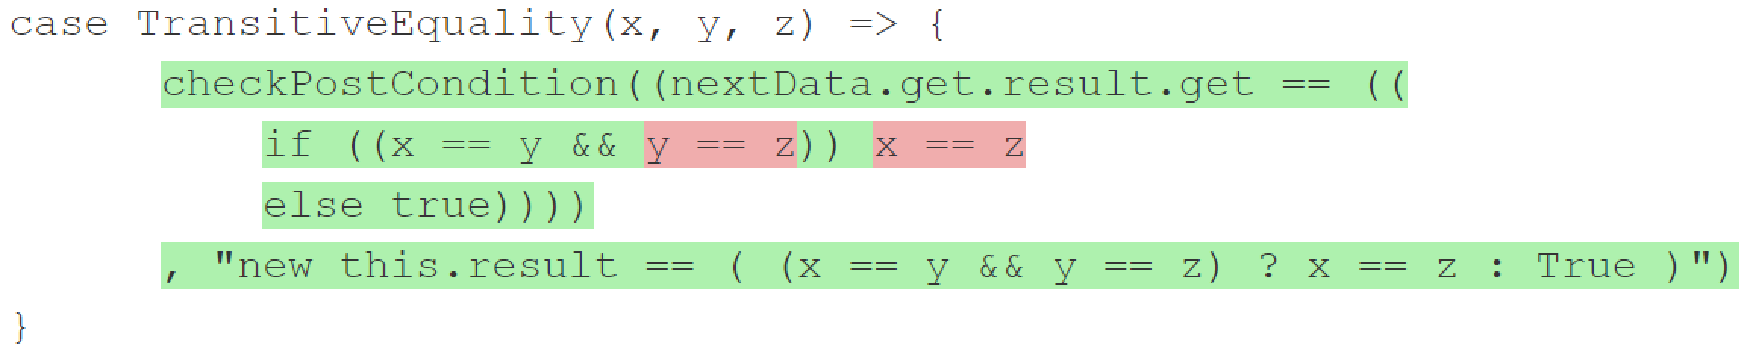
\includegraphics[width=\linewidth]{figures/e1_coverage_implicative_property}
%}
\caption{Test coverage of an implicative property (\textit{TransitiveEquality})}
\label{fig:experiment1_coverage_implicative_property}
\centering
\end{figure}
\FloatBarrier\noindent
% End figure

% Total coverage
The first criteria to evaluate an experiment was to determine the test
coverage. The implicative properties are not covered when using random
values as input data. The other properties, which do not use implication, are
fully tested though. In \autoref{fig:experiment1_evaluation_result} the results of the coverage report are shown, with a total of 87,80\% coverage. The file with its name
ending with ``Logic'' contain the implementation of the properties. The other 12,20\% code is not tested, but this part is also not related to the implementation of the properties. Because of this, it is not required to achieve the full 100\% coverage. Note that the coverage does not include the coverage over the libraries that the system uses. Some implementation details are depended on the libraries that the generated system use, thus it can not be concluded that 87,80\% of the system is now tested.
% Figure
\begin{figure}[!ht]
%\frame{
	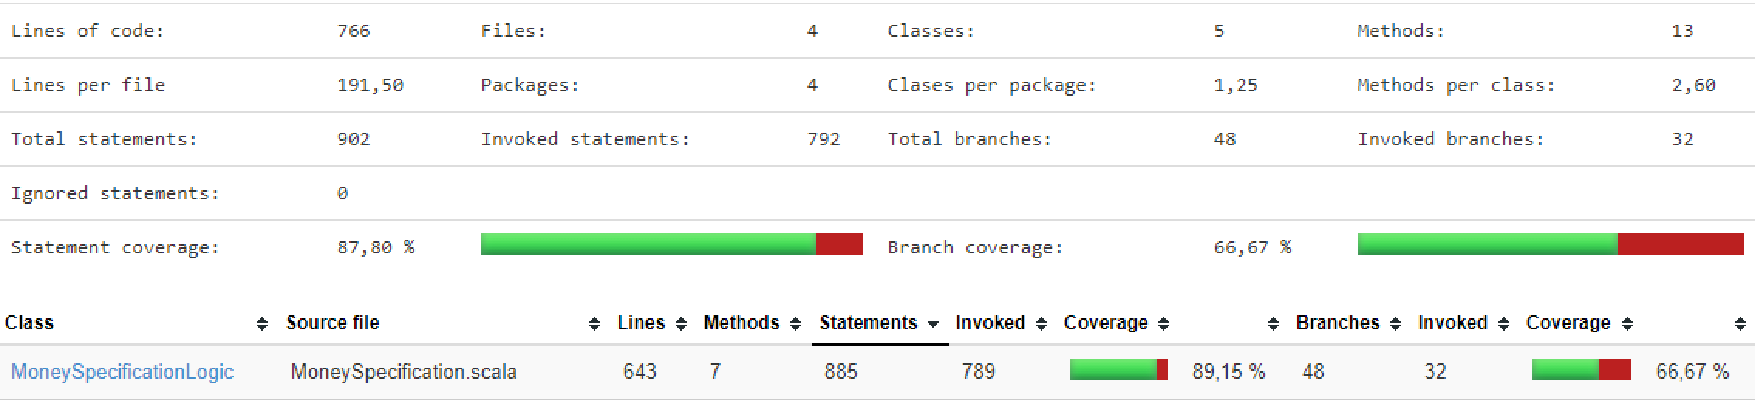
\includegraphics[width=\linewidth]{figures/eval_e1}
%}
\caption{Test coverage report of the first experiment}
\label{fig:experiment1_evaluation_result}
\centering
\end{figure}
\FloatBarrier\noindent
% End figure
The branch coverage is reported to be 66,67\%. This is caused by the implicative properties that are being translated to \textit{if-else} statements, where the \textit{else} branch is translated to \textit{true}. Furthermore the coverage could be increased as not every part of the condition of implicative properties are being checked, as we have seen in \autoref{fig:experiment1_coverage_implicative_property}.\\
\\
% % of bugs
\pinfo{\# of bugs, 8}
The second criterion that we defined is the number of bugs that we have found
by doing the experiment. By using this approach we found a total of 8 bugs. A
compilation error (1x), overflow/underflow errors (2x) and precision errors (5x). Many of these
precision errors originated from the library that is used for the \textit{Money}
type, for which we created an issue on
\textit{Github}\footnote{https://github.com/typelevel/squants/issues/265}. An
improvement to the test framework, such that the implicative properties are also covered, might
result in more bugs that can be found.

% % % % % % % % % % % % % % % % % % % % % % % % % % % % % % % % % % % % %
% Section: Conclusion
\section{Conclusion}
% 1: Squants using doubles internally. Small precision error can lead to bigger (unexpected) amounts as we've seen in AMP2.
% 	 - DistributivePercentage1: Multiplying Double with Money causes a precision error
%	 - DistributivePercentage2: Multiplying Money with Double causes a precision error
% 	 - DistributiveInt2: Multiplying Money with Integer
%    - AssociativeMultiplicationPercentage2: Multiplying Integer with Money. And with double. Causing big numbers to be losing precision anyway. Bug in Squants is the problem here though.
% 2: Operations on an Integer are over/underflowing, causing incorrect results.
%	 - AssociativeMultiplicationInt2: When using Multiply on Ints
%	 - DistributiveInt1: When using Addition on Ints
% 3: Percentage is double, causing big values to lose precision, which can cascade through the expressions
%	 - AssociativeMultiplicationPercentage1: Multiplying Percentage with Int, causing a big Double value with precision loss. Squants cannot guess the actual number anymore
\pinfo{Recap, found 8 bugs using this approach}
In this first experiment, we tested each property that was defined in
\autoref{cpt:properties} 100 times with using random values as input. First, the
test suite terminated due to a compilation error. After disabling the causing
property (temporarily), a total of 7 tests were failing. In this experiment, we
managed to find precision errors and overflow/underflow errors. Additionally, we
found a compilation error when using a property which was expected to hold. The
precision errors that were related to the \textit{Money} type were reported.
These bugs are fixed in the next version of the generator.\\
\\
\pinfo{Implicative properties not tested}
Although many properties were tested successfully, the test framework also
indicates that the implicative properties were satisfied. However, when looking
at the statement coverage of the implicative properties, we saw that the
if-clause is often not being triggered. Meaning that it would call the else-clause which
simply returns true. When relying on random data, there is a seldom chance that
the if-clause is being triggered. Thus we could optimize the generated input
values such that these satisfy the condition for the if-clause.

% % % % % % % % % % % % % % % % % % % % % % % % % % % % % % % % % % % % %
% Section: Threats to validity
\section{Threats to validity}

\subsection*{Fixed amount of tries}
\pinfo{Fixed amount of tries not substantiated}
The 100 tries to check a property is a fixed number that is being used. But why
exactly this number and not a higher or lower number? It might be the case that
some errors are not triggered because of this fixed amount. Running more cases
might be revealing an additional error, or it might not. In case it doesn't, it
means that the test framework just requires more time to run the whole test suite,
while it does not have an effect on the results. 100 seems to be an amount that
works such that it consistently reports the same amount of failing tests
however, this has checked by running it the test runs multiple times, also with
using numbers like 300 or 50 for the amount. Also \textit{QuickCheck} uses this
amount to check a property. During this thesis, we stick with 100 as the number
of tries. Finding the optimal number of tries is left as future work, thus
remaining as a threat to validity in this approach.\\
\\
The optimal amount of tries would be a useful addition when answering our second research question:\rqTwo Although we focus on automatically testing the properties, not mentioning the efficiency. But increasing the efficiency of the test framework would result in less time required to run it. Also, adding more properties would increase the time required to run the test suit. It might also be the case that increasing the number of tries would result in finding additional bugs. Thus leading to a threat to answering the third research question:\rqThree

\subsection*{Amount of test runs}
\pinfo{Multiple tries, each time 7 failed, assumed same causes}
The test framework has been executed several times for this experiment. With
each run, 7 tests were failing, which consistently were the same tests on every
run. Because of this, we assumed that the causes of these failures were the
same, as the same tests failed on each run. However, the causes might not have
been the same for these runs, thus remaining as a threat to validity to
answering our third research question. Because the causes of the failing tests
could be different and might reveal additional bugs.

\subsection*{Unfixed issue}
\pinfo{Compile error not fixed}
Unfortunately, the compilation error has not been fixed throughout this project
however, it is an open issue on
\textit{Github}\footnote{https://github.com/typelevel/squants/issues/281}. The
property causing this issue is disabled in order to continue running the test
framework. This prevents the test framework from detecting bugs that could be
found by this property.
